16. $y=\cfrac{x^2+5x+6}{|x+2|}=\cfrac{(x+2)(x+3)}{|x+2|}=\begin{cases} x+3,\ x>-2,\\ -x-3,\ x<-2.\end{cases}$
$$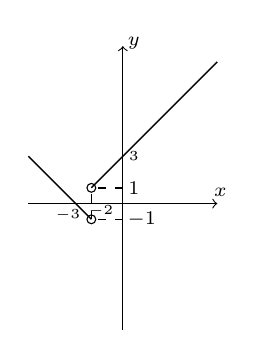
\begin{tikzpicture}[scale=0.2]
\tikzset {line01/.style={line width =0.5pt}}
\tikzset{line02/.style={line width =1pt}}
\tikzset{line03/.style={dashed,line width =0.5pt}}
%\filldraw [black] (0,0) circle (1pt);
\draw [->] (-6,0) -- (6,0);
\draw [->] (0,-8) -- (0,10);
\draw[line01] (-6,3) -- (-2,-1);
\draw[line01] (-2,1) -- (6,9);
\draw[line03] (-2,-1) -- (-2,1);
\draw[line03] (0,1) -- (-2,1);
\draw[line03] (0,-1) -- (-2,-1);
\draw (6.2,0.7) node {\scriptsize $x$};
\draw (1.2,-1) node {\scriptsize $-1$};
\draw (0.7,1) node {\scriptsize $1$};
\draw (0.7,3) node {\tiny $3$};
\draw (-1.4,-0.5) node {\tiny $-2$};
\draw (-3.5,-0.7) node {\tiny $-3$};
\draw (0.7,10.2) node {\scriptsize $y$};
\draw (-2,-1) circle (8pt);
\draw (-2,1) circle (8pt);
\end{tikzpicture}$$
